\documentclass[tikz]{standalone}
\usepackage[english]{babel}
\usepackage[T1]{fontenc}
\usepackage[utf8]{inputenc}
\usepackage[absolute,overlay]{textpos}
\usepackage{graphicx}
\usepackage[export]{adjustbox}
\usepackage{svg}
\usepackage{IEEEtrantools}
\usepackage{physics,dsfont,mathrsfs,cancel,tensor,slashed,mathtools}

\usepackage{amsmath}
\usepackage{amsfonts}
\usepackage{bm}
\usepackage{setspace}
\usepackage{subcaption}
\usepackage{mwe}
\usepackage{pgfplots}

\usepackage{tikz}
\usetikzlibrary{calc,patterns,decorations.pathmorphing,decorations.markings, angles, quotes}
\usetikzlibrary{arrows.meta}
\usepackage{tikzscale}

% ----------------------------
% Définition des nouvelles options xmin, xmax, ymin, ymax
% Valeurs par défaut : -3, 3, -3, 3
\tikzset{
xmin/.store in=\xmin, xmin/.default=-3, xmin=-3,
xmax/.store in=\xmax, xmax/.default=3, xmax=3,
ymin/.store in=\ymin, ymin/.default=-3, ymin=-3,
ymax/.store in=\ymax, ymax/.default=3, ymax=3,
}
% Commande qui trace la grille entre (xmin,ymin) et (xmax,ymax)
\newcommand {\grille}
{\draw[help lines] (\xmin,\ymin) grid (\xmax,\ymax);}
% Commande \axes
\newcommand {\axes} {
\draw [>=stealth,->] (\xmin,0) -- (\xmax,0);
\draw [>=stealth,->] (0,\ymin) -- (0,\ymax);
}
% Commande qui limite l’affichage à (xmin,ymin) et (xmax,ymax)
\newcommand {\fenetre}
{\clip (\xmin,\ymin) rectangle (\xmax,\ymax);}
% ----------------------------

\begin{document}

    %Paper figures
    % \documentclass[tikz]{standalone}% 'crop' is the default for v1.0, before it was 'preview'
% %\usetikzlibrary{...}% tikz package already loaded by 'tikz' option
% \begin{document}
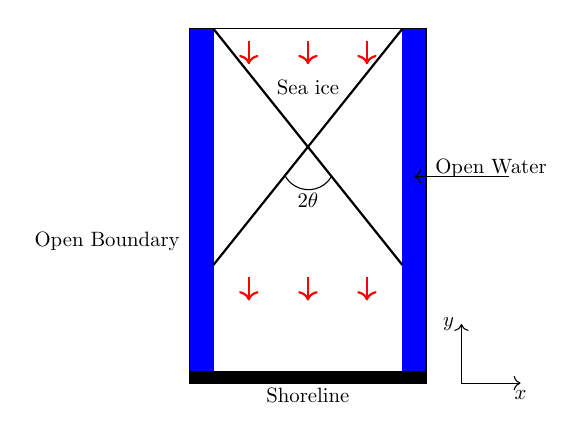
\begin{tikzpicture}[scale = 1.5]

   
    % \node at (1, -0.1) {\tiny Shoreline};

    \draw[->, thick, red] (0.5, 2.9) -- (0.5, 2.7);
    \draw[->, thick, red] (1, 2.9) -- (1, 2.7);
    \draw[->, thick, red] (1.5, 2.9) -- (1.5, 2.7);

    % \draw[->, thick, red] (0.5, 1.9) -- (0.5, 1.7);
    % \draw[->, thick, red] (1, 1.9) -- (1, 1.7);
    % \draw[->, thick, red] (1.5, 1.9) -- (1.5, 1.7);

    \draw[->, thick, red] (0.5, 0.9) -- (0.5, 0.7);
    \draw[->, thick, red] (1, 0.9) -- (1, 0.7);
    \draw[->, thick, red] (1.5, 0.9) -- (1.5, 0.7);

    
    \filldraw[blue] (0, 0) rectangle (0.2, 3);
    \filldraw[blue] (1.8, 0) rectangle (2, 3);
    \node[scale = 0.75] at (1, 2.5) { Sea ice};
    \node[scale = 0.75] at (1, -0.1) { Shoreline};
    \node[scale = 0.75] at (-0.7, 1.2) { Open Boundary};
   \node[scale = 0.75] at (2.55, 1.82) {Open Water};
    \filldraw (0,0) rectangle (2,0.1);
    \draw (0,0) rectangle (2,3);

    \draw[->] (2.7, 1.75) -- (1.9, 1.75) ;
    \draw[->] (2.3, 0) -- (2.8, 0) node[below, scale = 0.75] {$x$};
    \draw[->] (2.3, 0) -- (2.3, 0.5) node[left, scale = 0.75] {$y$};

    \draw[-, thick] (0.2, 3) -- (1.8, 1);
    \draw[-, thick] (0.2, 1) -- (1.8, 3);

    \draw  (1.2,1.75) arc[start angle = -30, end angle=-150,radius=0.225] ;
    \node[scale = 0.75] at (1, 1.55) {$2\theta$};
    
\end{tikzpicture}
% \end{document}


    
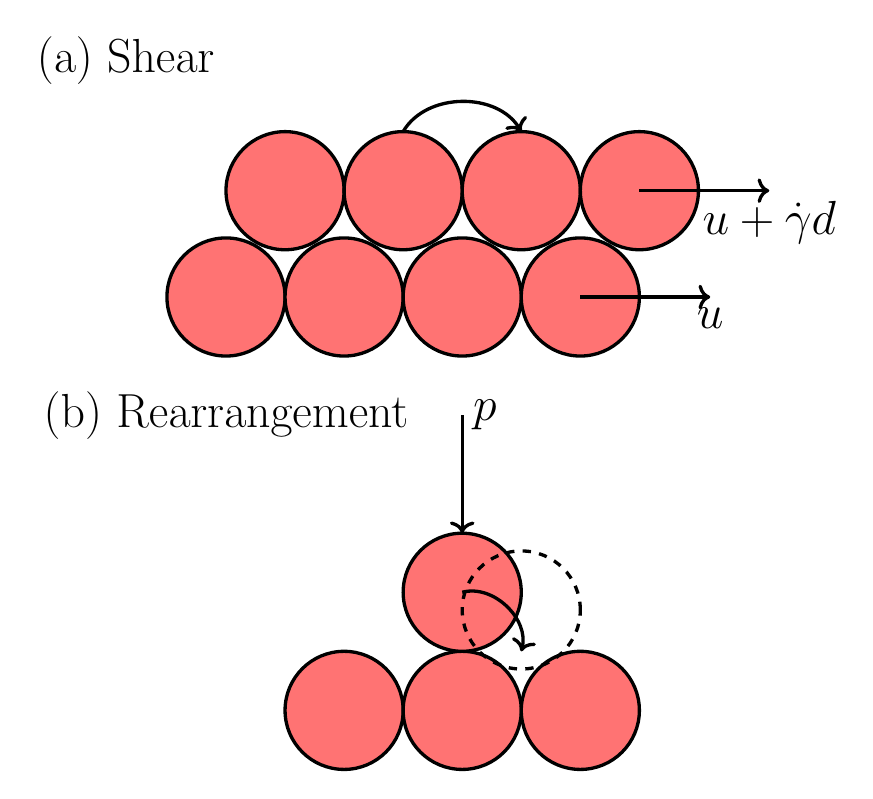
\begin{tikzpicture}[scale = 1.5]
    % \draw (-11.5,4) node {\textbf{A}};
    % \draw (-1.5,4) node {\textbf{B}};

    \def \b {3.5};
    \def \c {-7};
    \def \d {0.1};
    \def \r {0.5};
    \node at (1.15, 3)  {\LARGE (a) Shear};
    % \node at (2, 3.5)  {\LARGE $t_\text{macro} = 1/\dot{\gamma}$};
    % Before dilatancy
    \foreach \x in { 2, 3, 4, 5}
        \foreach \y in {1}
            \draw [color=black, fill=red!55,very thick] (\x, \y) circle (0.5);

    \foreach \x in { 2.5, 3.5, 4.5, 5.5}
        \foreach \y in {1.9}
            \draw [color=black, fill=red!55,very thick] (\x, \y) circle (0.5);
            
    \draw[->, very thick] (5, 1) -- (6.1, 1) node[below] {\LARGE $u$};
    \draw[->, very thick] (5.5, 1.9) -- (6.6, 1.9) node[below] {\LARGE $u + \dot{\gamma} d$};
    \draw[->, very thick, black] (3.5, 2.4) to [bend left=60] (4.5,2.4);

    \node at (2, 3.5-\b)  {\LARGE (b) Rearrangement};
    % Before dilatancy
    \foreach \x in { 3, 4, 5}
        \foreach \y in {1-\b}
            \draw [color=black, fill=red!55,very thick] (\x, \y) circle (0.5);

            \draw [color=black, fill=red!55,very thick] (4, 2-\b) circle (0.5);
            
    \draw [color=black,dashed,very thick] (4.5, 1.85-\b) circle (0.5);
    \draw[->, very thick, black] (4, 2-\b) to [bend left=60] (4.5,1.5-\b);
    \draw[->, very thick] (4, 3.5-\b) node[right] {\LARGE $p$}  -- (4, 2.5-\b) ;

    % \node at (2.2, 2.75-\b)  { \LARGE $t_\text{micro} = \overline{d}\sqrt{\frac{\rho_s}{p}}$};


\end{tikzpicture}



    

\begin{tikzpicture}
\begin{semilogxaxis}[
    xmode = log,
    log x ticks with fixed point,
    axis lines = left,
    log basis x=10,
    % grid=major
    xlabel = \(I\),
    ylabel = {\(\mu(I)\)},
    ymin = 0,
    ymax = 1,
    ymajorgrids=true,
    xmajorgrids=true,
    % xtickten={-7,...,0}
    % grid style=dashed,
]
%Below the red parabola is defined
\addplot [
    domain=10^-7:10, 
    samples=100, 
    color=red,
]
{0.1+(0.9-0.1)/(10^(-3)/x+1)};
% \addlegendentry{\(x^2 - 2x - 1\)}
%Here the blue parabola is defined

\end{semilogxaxis}
\end{tikzpicture}
% \end{document}

    
\begin{tikzpicture}[scale = 1.5]
    % \draw (-11.5,4) node {\textbf{A}};
    % \draw (-1.5,4) node {\textbf{B}};

    \def \b {8};
    \def \c {-7};
    \def \d {0.1};
    \def \r {0.5};

    % Before dilatancy
    \foreach \x in {1.1, 2.9, 4.7}
        \foreach \y in {1.5,..., 4.5}
            \draw [color=black, fill=red!55,very thick] (\x, \y) circle (0.5);

    \foreach \x in {2, 3.8}
        \foreach \y in {1,..., 4}
            \draw [color=black, fill=red!55,very thick] (\x, \y) circle (0.5);

    %contact forces
    \draw[ very thick, line width = 1mm] (2.9, 2.5) -- (2,3);
    \draw[ very thick,line width = 1mm] (4.7, 2.5) -- (3.8,3);
    
    \draw[dashed, very thick] (0, 5.03) -- (5.2,5.03);
    \draw[dashed, very thick] (0, 0.47) -- (5.2,0.47);

    \draw[->, very thick, line width = 1mm]  (0.1, 4.2) node[left] {\LARGE $p$} -- (0.1, 5.03) ;
     
    \draw [very thick, ->] (3, 5.3) -- (4.5, 5.3) node[above] {\LARGE Shear $\gamma$};


    \draw[->, line width = 2mm] (5.5, 3) -- (7.8,3);
    
    %When dilatating
    
    \foreach \x in {1.1, 2.9, 4.7}
        \foreach \y in {1.5,2.5}
            \draw [color=black, fill=red!55,very thick] (\x+\b, \y) circle (0.5);

    \foreach \x in {2, 3.8}
        \foreach \y in {1,2}
            \draw [color=black, fill=red!55,very thick] (\x+\b, \y) circle (0.5);

    \foreach \x in {2.9, 4.7}
        \foreach \y in {3.5, 4.5}
            \draw [color=black, fill=red!55,very thick] (\x+\b, \y) circle (0.5);

    \foreach \x in {2, 3.8, 5.6}
        \foreach \y in { 4,5}
            \draw [color=black, fill=red!55,very thick] (\x+\b, \y) circle (0.5);

    \draw[dashed, very thick] (0+\b, 0.47) -- (6+\b,0.47);
    \draw[dashed, very thick] (0+\b, 5.5) -- (6+\b,5.5);


    \draw[->, very thick, line width = 0.5mm]  (0.1+\b, 5.1) node[left] {\LARGE $p$} -- (0.1+\b, 5.5) ;
     
    \draw [very thick, ->] (3+\b, 5.7) -- (4.5+\b, 5.7) node[above] {\LARGE Shear $\gamma$};

    \draw[ very thick, line width = 0.5mm] (2.9+\b, 2.5) -- (2.9+\b,3.5);
    \draw[ very thick,line width = 0.5mm] (4.7+\b, 2.5) -- (4.7+\b,3.5);

    \coordinate (A) at (4, 2);
    \coordinate (B) at (2, 2);
    \coordinate (C) at (2.2, 2.4);
    \draw[dashed, thick, line width = 0.5mm] (2, 2) -- (3.5, 2);
    \draw[dashed, thick, line width = 0.5mm] (2, 2) -- (2.9, 3.5);
    \pic [draw, -,, angle eccentricity=1.5] {angle = A--B--C};
    
    \node at (1.9, 2.3)  {\LARGE $\psi $};
    \node at (0, 6)  {\LARGE (a) $\psi > 0$};




    \draw[->, line width = 2mm] (5.5, 3) -- (7.8,3);
    
    %When dilatating
    
    \foreach \x in {1.1, 2.9, 4.7}
        \foreach \y in {1.5,2.5}
            \draw [color=black, fill=red!55,very thick] (\x, \y+\c) circle (0.5);

    \foreach \x in {2, 3.8}
        \foreach \y in {1,2}
            \draw [color=black, fill=red!55,very thick] (\x, \y+\c) circle (0.5);

    \foreach \x in {1.3, 3.1}
        \foreach \y in {3.5, 4.5}
            \draw [color=black, fill=red!55,very thick] (\x, \y+\c) circle (0.5);

    \foreach \x in {2.2, 4 }
        \foreach \y in { 4,5}
            \draw [color=black, fill=red!55,very thick] (\x, \y+\c) circle (0.5);

    \draw[dashed, very thick] (0, 0.47+\c) -- (6,0.47+\c);
    \draw[dashed, very thick] (0, 5.5+\c) -- (6,5.5+\c);

    \coordinate (A) at (3.5, 3+\c);
    \coordinate (B) at (1.2, 3+\c);
    \coordinate (C) at (3.5, 2.2+\c);
    \draw[dashed,   very thick] (1.2, 3+\c) -- (3.5, 3+\c);
    \draw[dashed, very thick] (1.2, 3+\c) -- (3.5, 2.2+\c);
    \pic [draw, -,line width = 0.7mm, angle eccentricity=1.5] {angle = C--B--A};
    \node at (2.3, 2.8+\c) {\LARGE $\psi$};
    \draw[->, very thick, line width = 0.5mm]  (0.1, 5.1+\c) node[left] {\LARGE $p$} -- (0.1, 5.5+\c) ;
     
    \draw [very thick, ->] (3, 5.7+\c) -- (4.5+, 5.7+\c) node[above] {\LARGE Shear $\gamma$};

    \draw[ very thick, line width = 0.5mm] (1.1, 2.5+\c) -- (1.3,3.5+\c);
    \draw[ very thick,line width = 0.5mm] (2.9, 2.5+\c) -- (3.1,3.5+\c);

    \node at (0, 6+\c)  {\LARGE (b) $\psi < 0$};

    \foreach \x in {1.1, 2.9, 4.7 }
        % \foreach \y in {1,1.5, 2}
        \foreach \y in {1.5,..., 4.5}
            \draw [color=black, fill=red!55,very thick] (\x+\b, \y+\c) circle (0.5);

    \foreach \x in {2, 3.8}
        \foreach \y in {1,..., 4}
            \draw [color=black, fill=red!55,very thick] (\x+\b, \y+\c) circle (0.5);

    %contact forces
    \draw[ very thick, line width = 1mm] (1.1+\b, 2.5+\c) -- (2+\b,3+\c);
    \draw[ very thick,line width = 1mm] (2.9+\b, 2.5+\c) -- (3.8+\b,3+\c);
    
    \draw[dashed, very thick] (0+\b, 5.03+\c) -- (5.9+\b,5.03+\c);
    \draw[dashed, very thick] (0+\b, 0.47+\c) -- (5.9+\b,0.47+\c);

    \draw[->, very thick, line width = 1mm]  (0.1+\b, 4.2+\c) node[left] {\LARGE $p$} -- (0.1+\b, 5.03+\c) ;
     
    \draw [very thick, ->] (3+\b, 5.3+\c) -- (4.5+\b, 5.3+\c) node[above] {\LARGE Shear $\gamma$};
    
    
    \draw[->, line width = 2mm] (5.5, 3+\c) -- (7.8,3+\c);
\end{tikzpicture}




    
\begin{document}
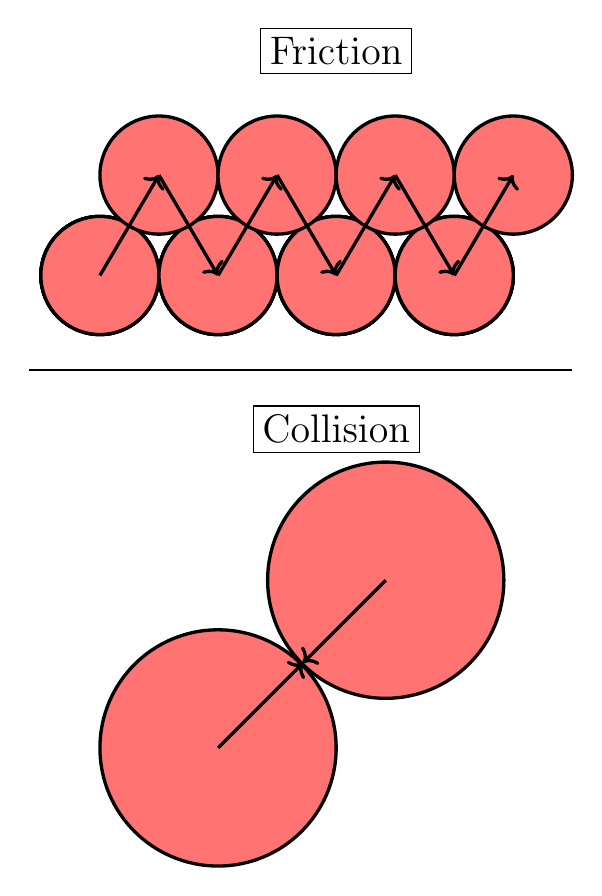
\begin{tikzpicture}[scale = 1.5]
    % \draw (-11.5,4) node {\textbf{A}};
    % \draw (-1.5,4) node {\textbf{B}};

    \def \b {-7};
    \def \c {0.1};
    \def \d {0.1};
    \def \r {2.3};

    \draw[color=black, fill=red!55, very thick] (-5, -3.7) circle (1);
    \draw[color=black, fill=red!55, very thick] (-5 + 1.42, 1.42-3.7) circle (1);
    \draw[->, very thick] (0-5, 0-3.7) -- (0.72-5, 0.72-3.7) ;
    \draw[->, very thick] (1.42-5, 1.42-3.7) -- (0.72-5, 0.72-3.7 );

    \node[draw] at (-4,2.2) { \Large Friction};
    \node[draw] at (-4,2.7-3.7) { \Large Collision};

    \foreach \x in {1, ..., 4}
        \foreach \y in {1.5, ..., 4.5}
            \draw [color=black, fill=red!55,very thick] (\x + \b, 0.3) circle (0.5);

            
    \foreach \x in {1.5, ..., 4.5}
            \draw [color=black, fill=red!55, very thick] (\x + \b, 1.15) circle (0.5);

    \foreach \x in {1, ..., 4}
            \draw [very thick, ->] (\x + \b, 0.3) -- (\x + \b + 0.5 , 1.15);

    \foreach \x in {1.5, ..., 3.5}
        % \foreach \y in {1, ..., 4}  
            \draw [->, very thick] (\x + \b, 1.15) -- (\x + \b + 0.5 , 0.3); 


    \draw [line width = 1pt] (-6.6,-0.5) -- (-2,-0.5); 

    
    % \foreach \x in {3, 4, ..., 5}
    %     \foreach \y in {0, 1, ..., 3}        
    %         \draw (\x - \d, \y - \c) circle (0.5);
\end{tikzpicture}


\end{document}